\section{Introdução} \label{sec:intro}

A crescente demanda por transição energética e pela descarbonização da economia impulsiona a busca por alternativas aos combustíveis fósseis nos setores de energia, transporte, indústria. 
Alguns setores, como o energético e o de transportes urbano de veículos leves, têm apresentado avanço significativo na utilização de energias renováveis e na eletrificação, respectivamente \cite{MasriA2021}. 
Porém, combustíveis fósseis são extremamente difíceis de substituir em outros setores, especialmente quando se trata de combustíveis líquidos.
Estes possuem maior energia específica e densidade energética \cite{Bergthorson2017,Julien2017} quando comparados com outras fontes de energia, como combustíveis gasosos ou baterias elétricas.
São assim adequados para aplicações de transporte, como no setor automotivo de cargas pesadas, naval e aeronáutico \cite{MasriA2021}.
Combustíveis líquidos são importantes também para algumas indústrias como aço e cimento, para algumas termoelétricas e até para máquinas portáteis movidas a motor de combustão interna (MCI).
Soma-se a isso uma análise histórica que indica que a transição para fontes renováveis se dará ao longo de décadas \cite{MasriA2021}.

% Nota-se que processos de combustão continuarão relevantes nas próximas décadas.
Todas as aplicações mencionadas anteriormente baseiam-se na combustão turbulenta de sprays líquidos.
Assim, é necessário buscar soluções que conciliem essa tecnologia com os esforços de transição energética e descarbonização da economia.
A comunidade científica e a indústria têm dado ênfase nas seguintes demandas: \textbf{(i)} desenvolver tecnologias para o uso de novos combustíveis (como  etanol, metanol, hidrogênio e amônia) \cite{MasriA2021,FAPESP_etanol_1,VerhelstS2019,TeohY2023,ElbazA2022}; \textbf{(ii)} desenvolver novas rotas de produção para combustíveis já utilizados (resultando, por exemplo, nos chamados SAF, biocombustíveis e eletro-combustíveis \cite{MasriA2021,BenJames-SAF,BergthorsonJ2015,WestbrookC2019,PalysM2022}); \textbf{(iii)} melhorar a eficiência dos \emph{"prime-movers"} a combustão e reduzir a formação de poluentes \cite{MasriA2021}.

Independente da origem do combustível, o processo de combustão deve ser bem compreendido para que \emph{"prime-movers"} e queimadores eficientes e com baixa emissão de poluentes sejam desenvolvidos.
Para tanto é necessário pesquisa em combustão, que pode ser estruturada em trabalhos experimentais e trabalhos de modelagem.
A modelagem da combustão turbulenta de sprays, foco dessa proposta, deve ser capaz de contemplar diferentes combustíveis líquidos, incluindo combustíveis oriundos das demandas (i) e (ii).
Deve também representar os diferentes fenômenos envolvidos nesse processo, como ignição e formação de poluentes, para atender a demanda (iii).
No âmbito da combustão turbulenta de sprays, é de extrema importância o modelo de transferência de calor e massa da gota (líquida) para a fase gasosa (HMT -\emph{Heat and Mass Transfer}).
Modelos HMT regem, dentre outros aspectos, a taxa de vaporização do combustível das gotas do spray.
É conhecido que essa modelagem tem enorme influência na chama \cite{JennyB2012}, afetando sua estrutura, distribuição de temperatura, geometria e formação de poluentes.


Nesse sentido, revisando a literatura mais recente, nota-se a necessidade de maior desenvolvimento de \textbf{modelos de evaporação e condensação} (MEC) computacionalmente eficientes capazes de representar corretamente diferentes combustíveis.
Por exemplo, modelos monocomponentes com equilíbrio termodinâmico, embora computacionalmente eficientes, não são capazes de representar todos os fenômenos associados à combustão de combustíveis hidrofílicos, como o etanol \cite{SacomanoF2024CF}, combustível de importância estratégica para o Brasil \cite{etanol-BNDES} e também para outros países, como a Índia \cite{etanol-India}.
Para descrever combustíveis comerciais como o etanol é necessário modelar a gota com abordagem de substância \textbf{multicomponente}, considerando \textbf{termodinâmica de mistura não-ideal} e os efeitos de transferência de calor e massa no \textbf{interior da gota} \cite{SacomanoF2024CF}.
% Em especial, nota-se uma demanda pela aplicação de modelos que tenham a capacidade de descrever diversos fenômenos subjacentes à combustão de sprays multicomponentes e computacionalmente robustos para serem utilizados na simulação de chama turbulenta de spray.  
% Em especial, nota-se uma demanda pela aplicação de modelos detalhados, desenvolvidos e testados em cenários simplificados, como na escala de uma única gota ou em simulações laminares ou unidimensionais, em simulações multidimensionais de combustão turbulenta.

Em MECs, a evaporação da gota fornece vapor de combustível que alimenta a chama.
Nessa abordagem, a chama não é estabilizada por uma gota em específica, mas se estabilizada por fenômenos específicos ao escoamento gasoso \cite{ChiuH1982,Law2006}.
Esse modo de combustão de spray é chamado \textbf{combustão com frente de chama externa}, ou simplesmente \textbf{combustão externa}.
Em contraste, é possível que as gotas entrem em combustão individualmente, com a evaporação de combustível alimentando uma frente de chama próxima e envolvente a cada gota, a uma distância na mesma ordem de grandeza que o diâmetro da gota \cite{ChiuH1977}.
Isso é chamado \textbf{combustão de gota isolada}.

Experimentos indicam que a combustão de gota isolada ocorre tanto durante a ignição	de sprays \cite{AggarwalS2014} quanto em sprays já desenvolvidos \cite{ChenG1996CF,SinghG2020,GounderJ2009PhD}.
Simulações DNS (\emph{Direct Numerical Simulation}) e LES (\emph{Large Eddy Simulation}) também indicam a ocorrência de combustão de gota isolada nessas duas etapas da combustão turbulentas de sprays líquidos, como em \cite{BorghesiG2013CF} e \cite{PaulhiacD2020,BojkoDesJardin2017CF}, respectivamente.
A combustão de gota isolada também ocorre na combustão de alguns pós metálicos como o alumínio \cite{Bergthorson2015,Julien2017,Baumann2020}, segundo várias evidências experimentais \cite{Braconnier2020Pre,Braconnier2022,Bucher1999,Halter2023}.
A Figura \ref{fig:sdc-exp} mostra evidências da combustão de gota isolada em sprays turbulentos de etanol (Figuras \ref{fig:GounderJ2009-7.17} e \ref{fig:SinghG2020-10}) e na combustão de uma partícula alumínio (Figura \ref{fig:Braconnier202PhD-5.20}). %\todo{explicar figuras ...}

Além disso, alguns trabalhos apontam para a combustão de gota isolada em sprays líquidos como uma fonte de emissão de fuligem \cite[e referências 3-13 \emph{loc. cit.}]{FachiniF2005}, de forma que a modelagem desse fenômeno contribui com os esforços de limitar as emissões de material particulado.

\begin{figure}[H]
    \centering
    \caption{Observações experimentais de combustão de gota isolada em chamas de etanol na Fig. \ref{fig:GounderJ2009-7.17} e \ref{fig:SinghG2020-10}, indicadas por setas, e ao redor de uma partícula de pó de alumínio na Fig. \ref{fig:Braconnier202PhD-5.20}. 
    Siglas: LIF -- \emph{Laser Induced Fluorescence}; HR -- \emph{Heat Release}.
    Adaptadas de \cite{GounderJ2009PhD,SinghG2020,Braconnier2020Pre}.
    }
    \begin{subfigure}[t]{0.39\textwidth}
        \centering
        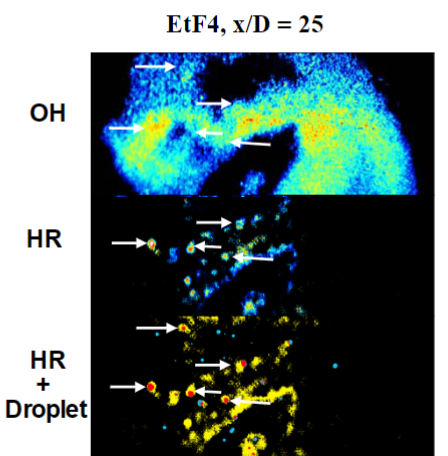
\includegraphics[width=0.99\textwidth]{30_images/GounderJ2009-7.17-1.png}
        \caption{LIF de OH, HR e HR sobreposto com posição das gotas em uma chama de etanol no queimador \emph{Sydney Dilute Spray Burner}, 25 diâmetros do injetor a jusante. Adaptado de \cite[Fig. 7.13]{GounderJ2009PhD}.}
        \label{fig:GounderJ2009-7.17}
    \end{subfigure}
    \hfill
    \begin{subfigure}[t]{0.59\textwidth}
        \centering
        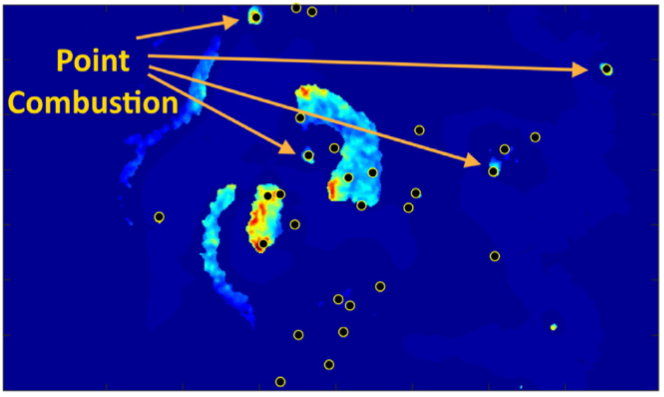
\includegraphics[width=0.99\textwidth]{30_images/SinghG2020-10.png}
        \vfill
        \caption{HR sobreposto com posição das gotas em uma chama de etanol no queimador \emph{Sydney Piloted Needle Spray Burner}, 20 diâmetros do injetor a jusante. Adaptado de \cite[Fig. 10]{SinghG2020}.}
        \label{fig:SinghG2020-10}
    \end{subfigure}
    \vspace{0.5cm}
    \begin{subfigure}[b]{0.8\textwidth}
        \centering
        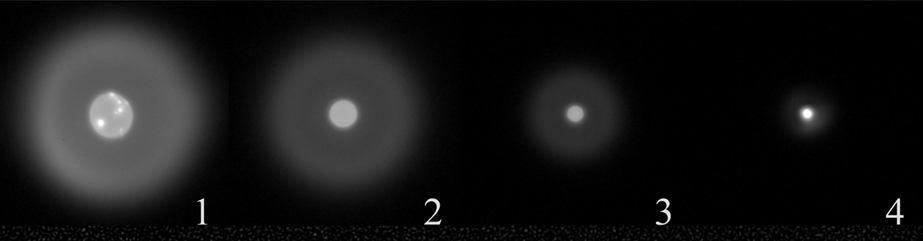
\includegraphics[width=0.99\textwidth]{30_images/Braconnier202PhD-5.20.png}
        \caption{Fotografias de combustão de uma partícula de alumínio de $\qntdd{50}{\mu m}$ de diâmetro em atmosfera 80\% Argônio/ 20\% oxigênio. Adaptado de \cite[Fig. 5.21]{Braconnier2022}.}
        \label{fig:Braconnier202PhD-5.20}
    \end{subfigure}
    \label{fig:sdc-exp}
\end{figure}

Diante dos aspectos expostos, constata-se que modelar a combustão de gota isolada é de grande importância para a descrição da ignição de sprays de combustíveis líquidos, da emissão de poluentes (em particular de fuligem) e também para a descrição da combustão de alguns combustíveis metálicos. 
Revisando a literatura, constatou-se a necessidade de desenvolver modelos de combustão de gota isolada (MCGI) capazes de representar corretamente diferentes combustíveis, incluindo as mesmas capacidades encontradas no chamado estado-da-arte para os MECs.
Notou-se também que não é claro na literatura quando a combustão de gota isolada ocorre \cite[p. 8]{JennyB2012} -- apesar de existirem diferentes modelos em cenários simplificados, a serem discutidos -- nem a influência de modelar a combustão de gota isolada (MCGIs) junto com a combustão externa (representada por MECs) na combustão turbulenta multidimensional.


\subsection{Objetivos} \label{sec:objetivos}

Tendo em vista os aspectos levantado anteriormente, este trabalho tem como objetivo avaliar os impactos do aumento de capacidade descritiva de modelos HMT em sprays multicomponentes e avaliar a influência da combustão de gota isolada na combustão de spray.
Para isso, esse trabalho propõe o desenvolvimento de estratégias para a simulação da transferência de calor e massa em gotas em dois cenários: (\textbf{A.}) combustão externa; (\textbf{B}.) combustão de gota isolada.
Esses cenários correspondem aos seguintes modelos HMT:
\begin{enumerate}
    \item[\textbf{A.}] Modelo de Evaporação e Condensação (MEC); e 
    \item[\textbf{B.}] Modelo de Combustão de Gota Isolada (MCDI).
\end{enumerate}
Esses modelos devem considerar os seguintes aspectos: 
\begin{enumerate}
    \item[\textbf{1.}] Descrição multicomponente da gota; 
    \item[\textbf{2.}] Gota com termodinâmica de mistura não-ideal; 
    \item[\textbf{3.}] Consideração dos efeitos de transferência	de calor e massa no interior da gota. 
\end{enumerate}
O objetivo é desenvolver aplicar a estratégia desenvolvida em simulações turbulentas reativas multidimensionais, com ambos modelos, {A} e {B} e com a funcionalidade:
\begin{enumerate}
    \item[\textbf{4.}] Determinação de quando ocorre a combustão de gota isolada;
\end{enumerate}
ou seja, de determinar se a gota se encontra no cenário {A} ou {B} e escolher o modelo apropriado para a correta representação dos fenômenos envolvidos.
Visando a aplicação em simulações CFD (\emph{Computational Fluid Dynamics}) turbulentas, reativas e multidimensionais, as estratégias a serem desenvolvidas devem ser robustas e computacionalmente eficientes.

O modelo HMT de simulações CFD que utilize as estratégias a serem desenvolvidas, incluindo as funcionalidades {1}, {2}, {3} e {4}, terá maior complexidade teórica em comparação aos modelos utilizados pela literatura. 
Isso permitirá ao autor dessa proposta investigar o efeito de considerar a combustão de gota isolada, e dos aspectos {1}, {2} e {3}, na estrutura da chama.
A investigação da estrutura da chama inclui a investigação de aspectos como distribuição de temperatura e concentrações de espécies, o que é essencial para a determinação da ignição, da eficiência de combustão e das emissões de poluentes.
% A relação da estratégia a ser desenvolvida \yellow{com a emissão de poluentes e com a ignição de sprays também será investigada.}